\providecommand{\CoverageVacuumDerivation}{Appendix~\ref{app:vacuum}}
\section{How far the improvement extends}
\label{sec:coverage}
The preceding gain was measured on known graph structures with a supplied master basis. To test its wider use, we now vary the physical structure as well as the loop order and include calculations that find their own basis. We keep the deployed models fixed so that these measurements test the current method on new inputs. The study contains 90 native-family requests, of which 54 fit the application's current index limit. It also tests a separate restricted vacuum construction at every loop order from one through twelve. This is a finite coverage study; a loop-order label alone does not establish coverage of all graphs at that order.

\subsection{Physical families and complete-time controls}
The native grid includes vacuum families with one or several masses, massless and massive two-point families, four-point ladders, and boxes with bubble subgraphs. We add planar, nonplanar, and five-point examples with independent symbolic kinematic parameters. Appendix~\ref{app:coverage} gives the denominator definitions, parameters, and targets. The 82 initial requests contain a sector-corner integral, one raised propagator power, and one numerator integral when an auxiliary denominator is available. Some massive two-point batches return every target unchanged as a master. We therefore preserve those results and add 8 separate batches containing every distribution of up to two dots over the physical denominators. The additional batches cover all six loop orders accepted for that two-point family, plus symbolic cases at one and two loops. Their inputs are fixed before their own comparison, and no model is refitted from either stage.

We first calculate a reference with expanded seeds and the revised implementation. A second calculation uses the previous executable and a larger numerator-rank bound, with the reference basis prescribed. Both must complete and reproduce the same coefficients before a case enters the repeated comparisons. This checks the reductions in the stated basis; it does not prove that the basis has the smallest possible size. Every native attempt has a 120-second allowance, a 6 GiB address-space limit, and a 5,200 MiB process-tree memory limit. An attempt that reaches a limit remains a failed result. Inputs with more than 31 indices exceed the current application's accepted domain and receive no timing estimate.

The first comparison runs the saved original Kira executable, the previous improved implementation, and the revised implementation with the same expanded seed region. These calculations receive no master list, so their times include basis discovery, equation generation, elimination, coefficient checks, and cleanup. This comparison measures the complete effect of the implementation. It makes no learned decision. The second comparison supplies the checked basis and runs the previous learned application, the revised learned application, and a native-choice control with revised preparation. Its times also include prediction and unsuccessful attempts. Both comparisons use three repetitions with rotated method order and fresh Kira processes. Initial caller imports and model loading remain separate from the repeated application times.

An input audit finds two box-with-bubble definitions that match saved training structures exactly but carry new family names. The initial application treats these names as unknown. We add a lookup that resolves a unique match of the ordered momentum forms, sector definition, and zero or nonzero mass pattern before prediction. Numerical mass and kinematic values remain free, as in the existing model signature, and all original feature-range checks remain active. Unmatched structures retain the native fallback. The lookup uses no measured time or reference coefficient. We repeat the paired application comparison for both names and use these corrected pairs in the application totals. The initial unknown-name measurements remain available separately. This correction allows the existing models to recognize their own domain; it does not train a new model or infer equivalence between different momentum representations.

\subsection{Coverage and measured time}
Figure~\ref{fig:coverage-grid} shows the rational grid, including its failures and unsupported inputs. The reference checks pass for 41 requests, and 41 requests complete all three revised full-calculation repetitions. Of these, 39 contain a nontrivial reduction and 2 contain only identity outputs. We exclude identity-only requests from speedup ratios. The supplied-basis selected application completes all repetitions for 41 requests. The remaining requests retain their stated failure or support-limit classification. The timings therefore do not establish a nontrivial reduction for every entry in the grid.

\begin{figure}[!htbp]\centering
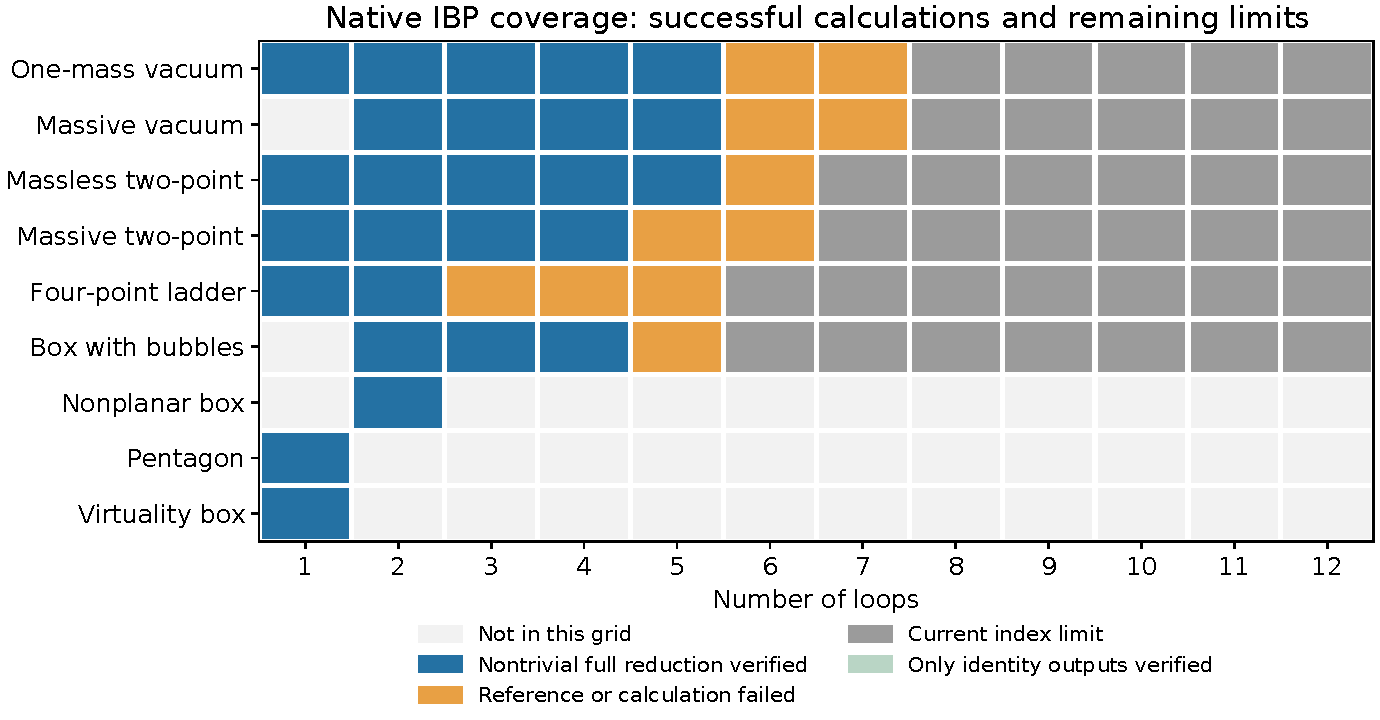
\includegraphics[width=\linewidth]{paper_figures/coverage_grid.pdf}
\caption{Native IBP coverage in the rational grid. Blue requires a checked reference, a nontrivial reduction, and three exact revised full calculations including basis discovery. Pale green records only identity outputs. Orange records a failed reference or calculation within the stated limits. Gray records the current index limit. A cell takes the strongest verified status across initial and additional batches. Blank cells are absent from this grid; the two coincident one-loop definitions appear only once. Symbolic requests enter the timing table and the text totals.}
\label{fig:coverage-grid}
\end{figure}

Table~\ref{tab:coverage-times} uses a separate matched set for each comparison. A request enters a row only when both methods complete all repetitions and the reduction contains a nontrivial coefficient. We sum the median time of each request, so a smaller ratio means less total time on that completed set. The revised full calculation takes 88.2\% less time than the saved original Kira executable and 54.3\% less time than the preceding improved implementation on their respective matched sets. The supplied-basis selected application takes 54.1\% less time than the previous application and 0.1\% less time than the revised native control. These aggregates retain slower individual requests and do not turn unsuccessful cases into speedup estimates.

\begin{table}[!htbp]\centering\small
\caption{Summed request median times in seconds. The revised column uses full revised calculations for the first two rows and the selected application for the last two. Each row names its own control and completed request count.}
\label{tab:coverage-times}
\begin{tabular}{@{}lrrrr@{}}\toprule
Control & Requests & Control time & Revised time & Ratio\\\midrule
Full: original Kira & 37 & 369.363 & 43.750 & 0.118\\
Full: previous implementation & 39 & 146.541 & 66.897 & 0.457\\
Basis supplied: previous application & 39 & 146.342 & 67.195 & 0.459\\
Basis supplied: revised native control & 39 & 67.269 & 67.195 & 0.999\\
\bottomrule\end{tabular}
\end{table}

The revised native control passes through the same input checks and portfolio proposal before overriding the proposed action. For a conservative comparison, we subtract that entire recorded interval and the family-name lookup from its time, while retaining every selected-application cost. The largest removed interval is 2.124 milliseconds. This gives an optimistic native total of 67.259 seconds, against which the selected application takes 0.1\% less time. The subtraction also removes useful input checks, so it supplies a sensitivity bound rather than a separately timed implementation.

The selected application and revised native control differ by only 0.1\% in the summed medians. With only three repetitions, this small difference does not establish a reliable additional learned gain on the wider grid. The larger improvement against the preceding application includes the exact preparation changes.

The repeated native comparisons contain 752 recorded requests, with 750 exact completions and 2 unsuccessful requests. The largest recorded process-tree memory use among these timings is 961.8 MiB. The grid includes new graph definitions, so the existing domain guard often retains native choices. This is part of the deployed method and prevents us from describing the full implementation gain as a gain from newly learned decisions.

Table~\ref{tab:coverage-completion} also includes unsuccessful first timed requests. Its elapsed totals describe the cost actually incurred on that common reference-verified collection. They are not completed-reduction speedups, since a failed request supplies no accepted answer. This view complements the paired timing table and prevents completion failures from disappearing in an aggregate improvement claim.
\begin{table}[!htbp]\centering\small
\caption{First timed requests on the reference-verified collection. Elapsed seconds include failed requests. Later repetitions are excluded from this table so that each method receives one request per case.}
\label{tab:coverage-completion}
\begin{tabular}{@{}lrrr@{}}\toprule
Method & Requested & Exact completions & Elapsed seconds\\\midrule
Full original Kira & 41 & 39 & 623.836\\
Full previous implementation & 41 & 41 & 148.606\\
Full revised implementation & 41 & 41 & 68.568\\
Previous application & 41 & 41 & 150.733\\
Selected application & 41 & 41 & 68.497\\
Revised native control & 41 & 41 & 68.721\\
\bottomrule\end{tabular}
\end{table}

\subsection{Every tested loop order in the restricted vacuum class}
The existing vacuum recurrence has a different domain: unit powers on the massless lines and several massive denominators with the same total loop momentum. We construct three new mass profiles with two, three, or four distinct masses and six target exponent vectors per profile. We compare the saved original Kira, dense and selected supplied-identity systems, the frozen learned identity selector, and the deployed exact recurrence. Each method receives the same targets and passes the independent coefficient check derived in \CoverageVacuumDerivation{}. The individual requests cover every loop order from one through twelve. Separate shared requests ask for all twelve orders together.

The study records 585 exact completions in 585 vacuum requests. Table~\ref{tab:coverage-vacuum} separates individual-loop requests from shared requests. In the individual-loop set, learned identity selection takes 8.2\% more time than the fixed identity rule. The deployed recurrence takes 99.8\% less time than the saved original Kira calculation. This gain uses the exact restricted-family relations and their implementation; the deployed recurrence uses its existing fixed policy. The native study and this supplied-identity study therefore establish different forms of coverage.

\begin{table}[!htbp]\centering\small
\caption{Restricted vacuum timings in seconds, summed over request medians. There are 36 individual-loop requests and three shared requests, each repeated three times. The original control solves separately for each requested loop order. The other methods can use the exact shared variable $z=L(d-2)$. All times include coefficient verification.}
\label{tab:coverage-vacuum}
\begin{tabular}{@{}lrr@{}}\toprule
Method & Individual loops & Shared loops\\\midrule
Original Kira, separate loop orders & 122.179 & 129.306\\
Improved Kira, dense identities & 14.626 & 1.310\\
Fixed identity selection & 13.311 & 1.398\\
Learned identity selection & 14.399 & 1.327\\
Deployed exact recurrence & 0.189 & 0.069\\
\bottomrule\end{tabular}
\end{table}

\begin{figure}[!htbp]\centering
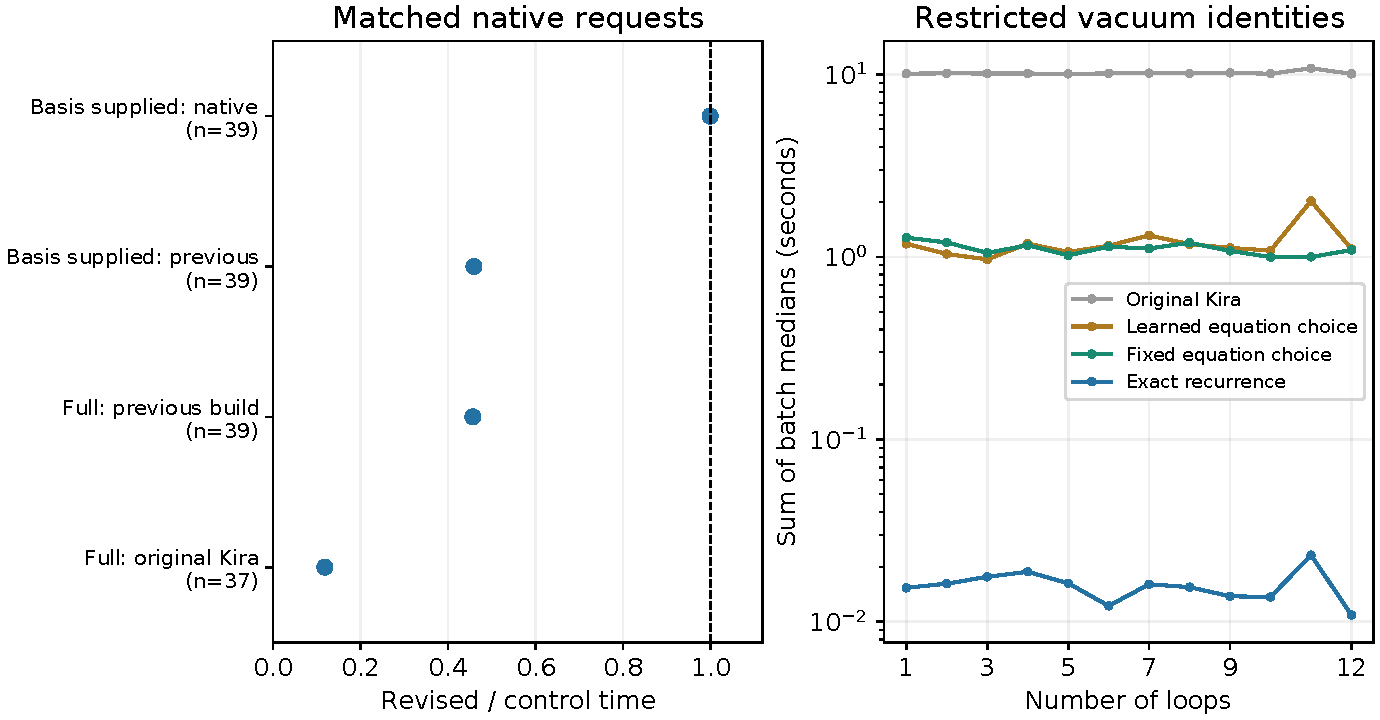
\includegraphics[width=\linewidth]{paper_figures/coverage_times.pdf}
\caption{Left: revised-to-control time ratios on matched completed native requests; the dashed line marks equal time. The request count changes with each pair's completed coverage. Right: restricted vacuum time at each loop order, summed over the three mass profiles. The logarithmic vertical axis keeps the exact recurrence and Kira-based calculations visible. These panels use different integral definitions and cannot be combined into a universal speedup.}
\label{fig:coverage-times}
\end{figure}

The broader tests identify where the current application completes an exact reduction, where its cost changes, and where its support or resource limits stop the calculation. They retain the earlier known-graph gain while restricting its interpretation to measured inputs. General high-loop scattering, arbitrary numerator rank, cuts, symbolic propagator powers, and every possible mass or kinematic assignment remain outside a universal verified claim.
